\subsection{Variation und Kombination \hfill IP}
\begin{scriptsize}
    \begin{center}
        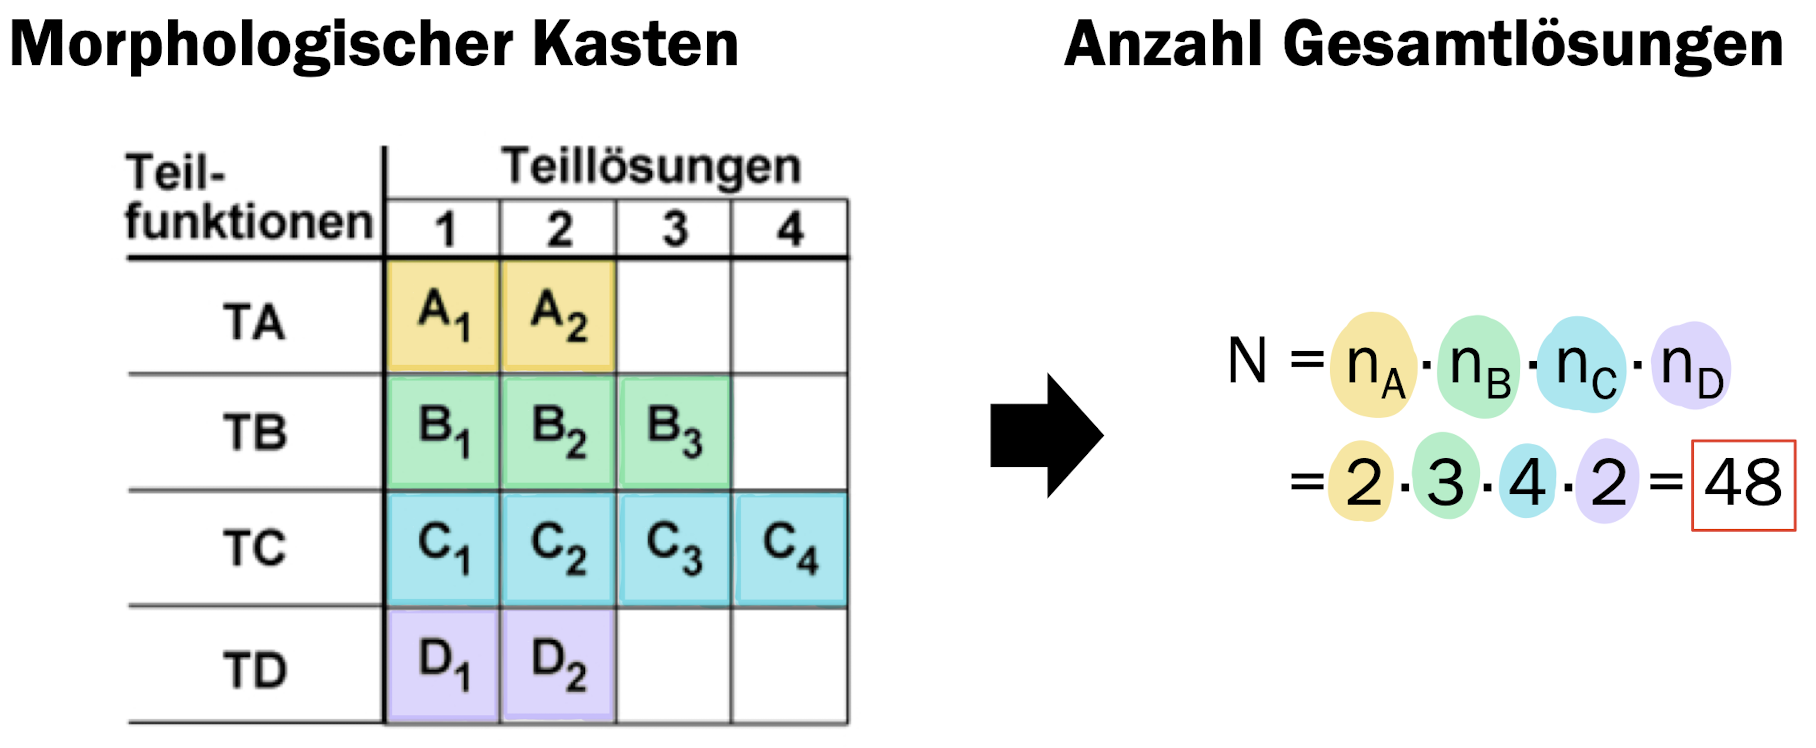
\includegraphics[width = 0.8\linewidth]{src/images/MAEIP_MorphologischerKasten}
    \end{center}
    \begin{empheq}[box=\fbox]{align*}
        &\textbf{Wenn \# unverträglicher} \: \textbf{Kombinationen = 1:} 
        \\ &n_{\text{unverträglich}} = \frac{N_{\text{max}}}{(n_x \cdot n_y)}
        \\ &n_x \& n_y := \text{Anzahl Teillösungen der betroffenen Teilfunktionen}
        \\ & \textbf{Wenn \# unverträglicher Kombinationen $>$ 1: } 
        \\ &\text{Variantenbaum aufstellen}
    \end{empheq}
\end{scriptsize}